\documentclass[10pt]{beamer}

%% Use this for 4 on 1 handouts
%\documentclass[handout]{beamer}
%\usepackage{pgfpages}
%\pgfpagesuselayout{4 on 1}[landscape, a4paper, border shrink=5mm]

\usepackage[english]{babel}
\usepackage[latin1]{inputenc}
\usepackage[T1]{fontenc}
\def\subitem{\item[\hspace{1.5cm} -]}

\usepackage{graphvizzz}

% Set the presentation mode to BTH
\mode<presentation>
{
	\usetheme{BTH_msv}
	% Comment this if you do not want to reveal the bullets before they are going to be used
	\setbeamercovered{transparent}
}


% Information for the title page

\title[]{Quality Attributes}
%\date[]{}

\author[Mikael Svahnberg]{Mikael Svahnberg\inst{1}}
\institute[BTH] % (optional, but mostly needed)
{
  \inst{1}%
 Mikael.Svahnberg?bth.se\\
 School of Computing\\
 Blekinge Institute of Technology%
}

% Delete this, if you do not want the table of contents to pop up at
% the beginning of each subsection:
%\AtBeginSubsection[]
%{
%  \begin{frame}<beamer>{Outline}
%    \tableofcontents[currentsection,currentsubsection]
%  \end{frame}
%}


% If you wish to uncover everything in a step-wise fashion, uncomment
% the following command: 
%\beamerdefaultoverlayspecification{<+->}

\begin{document}

% Titlepage frame
\begin{frame}
  \titlepage
\end{frame}

% ToC frame
% Use \section and \subsection commands to get things into the ToC.
%\begin{frame}
 %\frametitle{Outline}
 % \tableofcontents
%\end{frame}

% -----------------------------
% Your frames goes here
% -----------------------------

\begin{frame}[t]
\frametitle{Quality}

\begin{itemize}
\item What is quality?
\end{itemize}

\end{frame}

\begin{frame}[t]
\frametitle{Requirement vs Attribute}
\begin{itemize}
\item A quality attribute is always present
\item A quality requirement puts a constraint on an attribute
\item A quality requirement describes a service level of the system (or, more likely, a functional requirement).
\end{itemize}
\end{frame}

\begin{frame}[t]
\frametitle{Architecture and Quality Attributes}
\begin{itemize}
\item Functionality is ``easy'' to implement.
\item Quality requirements may \emph{sometimes} have impact on the implementation
\item More often, it impacts the \emph{software structure} (=the software architecture).
\item \ldots And yet, the architecture can only describe a \emph{potential} for achieving a particular quality level.
\end{itemize}
\end{frame}

\begin{frame}[t]
\frametitle{Examples}

\begin{itemize}[<+->]
\item Usability
\begin{itemize}
\item $\neg$Button layout etc.
\item Certain functions (e.g. undo, data re-use).
\end{itemize}
\item Modifiability
\begin{itemize}
\item How is functionality divided?
\item \ldots In relation to likely change scenarios.
\end{itemize}
\item Performance
\begin{itemize}
\item communication between components
\item division of functionality between components
\item allocation of shared resources
\item $\neg$choice of algorithms
\end{itemize}
\end{itemize}
\end{frame}

\begin{frame}[t]
\frametitle{Levels of Quality Attributes}
\begin{itemize}
\item Business Qualities
\begin{itemize}
\item Time-to-Market, Cost and Benefit, Projected Lifetime, Targeted market, Rollout schedule, Legacy system integration
\item Also: Product portfolio, Requirements from Society, etc.\footnote{T. Gorschek and A. M. Davis. Requirements engineering: In search of the dependent variables. \emph{Information and Software Technology}, 50(1-2):67-75, 2008.}
\end{itemize}
\item System Quality Attributes
\begin{itemize}
\item Availability, Modifiability, Performance, Security, Testability, Usability
\item ISO 9126: Functionality, Reliability, Usability, Efficiency, Maintainability, Portability
% \item There are many more classifications. See e.g. Svahnberg \& Henningsson 2009\footnote{M. Svahnberg and K. Henningsson. Consolidating different views of quality attribute relationships. In \emph{7th Workshop on Software Quality, proceedings of the International Conference on Software Engineering (ICSE2009)}, pages 46-50, Los Alamitos CA, may 2009. IEEE Computer Society Press.}
\end{itemize}
\item Architecture Qualities
\begin{itemize}
\item Conceptual Integrity, Correctness and Completeness, Buildability
\end{itemize}
\end{itemize}
\end{frame}

\begin{frame}[t]
\frametitle{Achieving Quality Attributes (I)}
\begin{itemize}
\item In order to achieve a a certain level for a quality attribute we need a \emph{controlled process} to lead us towards an architecture \emph{decision}.
\item Quality Attribute Scenarios is one building block for this:
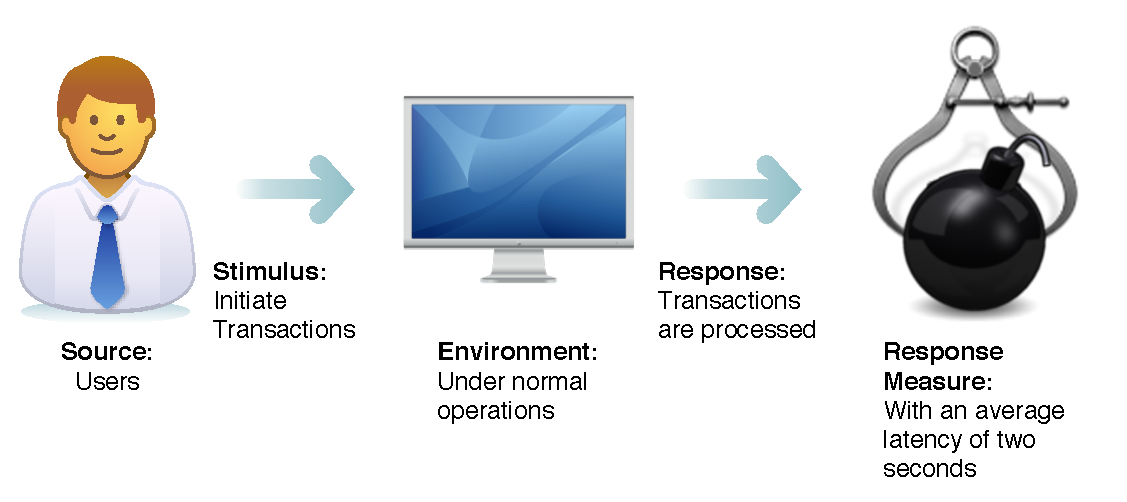
\includegraphics[width=10cm]{IQAScenario.pdf}
\end{itemize}
\end{frame}

\begin{frame}[t]
\frametitle{Example of Quality Attribute Scenario: Performance}
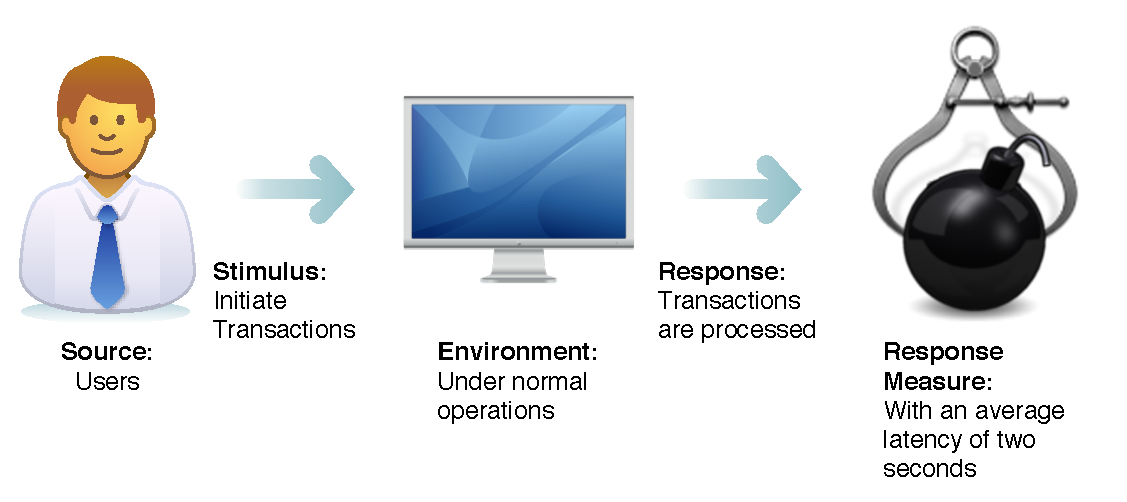
\includegraphics[width=10cm]{IQAScenario.pdf}
\begin{scriptsize}
\begin{tabular}{ll}
Aspect & Value\\
\hline
Source & Users\\
Stimulus & Initiate transactions: 1000 per minute\\
Artifact & System\\
Environment & Normal mode (c.f. overload mode)\\
Response & Transactions are Processed\\
Response Measure & Latency of 2s (deadline, throughput, jitter, miss rate, data loss, etc)\\
\hline
\end{tabular}
\end{scriptsize}
\end{frame}

\begin{frame}[t]
\frametitle{Achieving Quality Attributes (II)}
\begin{itemize}
\item The next step is to find a solution to a Quality Attribute Scenario.
\item To this, we have \emph{tactics}.
\item A tactic \emph{can be} (but is not limited to) a design pattern, an architecture pattern, or an architectural strategy.
\end{itemize}
\end{frame}

\begin{frame}[t]
\frametitle{Other Concerns}
\begin{itemize}
\item One may be led to believe that if only the quality requirements are taken care of, the rest will follow.
\item Obviously, this is not the case.
\item Hofmeister et al.\footnote{C. Hofmeister, R. Nord, and D. Soni. \emph{Applied Software Architecture}. Addison-Wesley, Reading MA, 2000.} lists three sources of concerns\footnote{Please note the overlap to the categories from Bass et al.}:
\begin{itemize}
\item Organisational factors:
\only<1>{
\begin{itemize}
\item Management (cf. business qualities above)
\item Staff skills, interests, strenghts, weaknesses
\item Process and development environment
\item Development schedule
\item Development Budget
\end{itemize}
}
\item Technological factors
\only<2>{
\begin{itemize}
\item General-purpose hardware
\item Domain-specific hardware
\item Software technology
\item Architecture technolog
\item Standards
\end{itemize}
}
\item Product factors
\only<3>{
\begin{itemize}
\item Functional Features
\item User Interface
\item Performance
\item Dependability
\item Failure detection, reporting, recovery
\item Service
\item Product cost
\end{itemize}
}
\end{itemize}
\end{itemize}
\end{frame}

\begin{frame}[t]
\frametitle{Software Solutions}
\begin{itemize}
\item In a course (or any hypothetical system that is never going to be built), it is often easy to solve issues simply by allowing more or better hardware.
\item In industry, the hardware constraints are \emph{real} and \emph{hard}.
\item For example (using low estimates):
\begin{itemize}
\item Require 1GB more internal memory in the computer = 17 Euro.
\item Ship 1000 units/year = 17 000 Euro.
\item Expected lifespan of system: 10 years = 170 000 Euro.
\item Ensure availability of the right memory modules for the hardware platform for the coming 10 years: lots more.
\end{itemize}
\item Contrast this with one well payed swedish developer working full-time for one year to reduce the memory consumption in software: 75000 Euro (including tax and social fees).
\end{itemize}
\end{frame}


% -----------------------------

\begin{frame}[t]
\frametitle{Architectures for different purposes}

\begin{itemize}
\item Regular desktop applications
\item Embedded applications
\item Enterprise applications
\item Applications for Android / IOS
\item Cloud applications
\item Service-Oriented Architectures (SOA)
\item Software Ecosystems
\item \ldots
\end{itemize}
\end{frame}

\begin{frame}[t]
\frametitle{What can differ?}
\begin{itemize}[<+->]
\item Instantiation into different viewpoints?
\subitem Trivial, the views will differ between each application anyway.
\item Factors, Issues and Strategies?
\subitem Also trivial, for the same reason.
\item The \emph{importance} of certain factors (e.g. the importance of certain quality requirements).
\item \emph{Typical choices} of strategies for a particular domain.
\item Typical choices of architecture styles for a particular domain (may be subordinate to the aforementioned)
\end{itemize}
\end{frame}

\begin{frame}[t]
\frametitle{Embedded Applications I}
This is a large and diverse field, and there are many quality requirements that may be in focus for different applications. However, there are some overall constraints that hold true for \emph{most} applications in this domain:
\begin{itemize}
\item {\bf Hardware cost} %See the example in L02; You may think that if you have a 5M\$ container AGV, the cost of the control module is inconsequential, but every cent counts.
\subitem Keep memory footprint low
\subitem Keep CPU usage low
\subitem Optimise for wear and tear
\item {\bf Hardware availability for entire product life expectancy} %Ensuring that a particular piece of hardware works in your operating environment, and \emph{guaranteeing} this, is expensive. Therefore you are often locked to a particular hardware platform for a long, long time. today, 80486 CPUs are often used in embedded applications, along with Motorola 68000. When did you last own a desktop computer with any of these?
\subitem Keep memory and CPU usage low.
\subitem Cull system regularly to remove stuff that is no longer needed.
\subitem Low-cost growth mechanisms.
\end{itemize}
\end{frame}

\begin{frame}[t]
\frametitle{Embedded Applications II}
\begin{itemize}
\item {\bf Testability} %This is connected with reliability since your ability to do product upgrades is limited (or even undesired by many customers). You must ensure that your product works as specified prior to release.
\subitem Testable software -- the usual stuff
\subitem Testable hardware -- system test software, test harness, etc.
\subitem Report error states (e.g. through flashing diodes).
\item {\bf Reliability} % Goes hand in hand with testability. Once you have released, it had better work, since the error reporting facilities are limited. Can often be safety critical applications or stowed away somewhere inaccessible.
\subitem Error detection
\subitem Error recovery
\subitem Report error states visibly (e.g. on-line, flashing diodes)
\end{itemize}
\end{frame}

\begin{frame}[t]
\frametitle{Embedded Applications III}
\begin{itemize}
\item {\bf Energy consumption} % Handheld devices are obvious, but consider an AGV. If you can reduce battery consumption by, say 10\%, then you can deploy that vehicle 10/% more, and you do not have to drive it back to the charging station (which, in turn, recudes wear and tear as well as traffic and battery life (that is affected by the number of chargings).
\subitem Low-effort computing
\subitem Reduce display time and display size (if any)
\subitem Powersave modes
\subitem Lazy evaluations -- deferred processing
\item {\bf Network communications} % Especially for embedded systems that consist of several communicating devices.
\subitem Standard communications platform
\subitem Robust transfers (e.g. in outdoor environments)
\subitem Operate by ``dead reckoning''
\end{itemize}
\end{frame}

\begin{frame}[t]
\frametitle{Enterprise Applications I}
\begin{itemize}
\item Enterprise architectures only has very little to do with software architecture -- and yet it has \emph{everything} to do with the software architecture.
\item Organisational, Technological, and Product factors can be considered subsets, or limited views, of the enterprise architecture.
\end{itemize}
\end{frame}

\begin{frame}[t]
\frametitle{Enterprise Applications II:\\List of Concerns}
\begin{itemize}
\item Persistent Data\footnote{M. J. Fowler. \emph{Patterns of Enterprise Application Architecture}. Addison-Wesley, Boston MA, 2003.}
\item Large amounts of data
\item Large scale concurrent access
\item Many data views (user interface screens)
\item Need to integrate with other enterprise applications
\item Multiple interpretations of data (conceptual dissonance)
\item Complex business logic rules (business ``illogic'')
\item Various types of enterrpise systems $\{B,C\}2\{B,C\} \wedge B,C \in \{s,m,l,xl,xxl\}$
\end{itemize}
\end{frame}

\begin{frame}[t]
\frametitle{Enterprise Applications IV:\\Typical Architecture Styles}
\begin{itemize}
\item Function-centric (Transaction script)
\item Domain concept-centric (Domain model)
\item Data representation-centric (Table module)
\end{itemize}

\ldots I could go on, but the book (Fowler 2003) is rather thick and full of patterns that dig deeper and deeper into the application.
\end{frame}

\begin{frame}[t]
\frametitle{Android/IOS Applications}
Somewhere between embedded and desktop applications. Any number of quality concerns may be relevant for any application. The platform itself imposes some concerns.
\vspace{0.5cm}
\begin{scriptsize}
\begin{columns}[t]
\column{5cm}
Hardware:
\begin{itemize}
\item Restrict battery usage
\item Small screen%, limited space for data presentation.
\item Unorthodox input methods (e.g. thumb)
\item Not the fastest CPU, restricted RAM.
\item Variety of hardware available on a particular phone model.
\end{itemize}
%
\column{5cm}
Software:
\begin{itemize}
\item Interruptible applications (e.g. for phone calls)
\item Interoperable applications
\item Reuse wherever possible, yet enable customisation.
\item Intuitive user experience that supports how users operate their handheld device (e.g., avoid deep meny hierarchies).
\item Varity of services available on a particular phone.
\end{itemize}
\end{columns}
\end{scriptsize}
\end{frame}

\begin{frame}[t]
  \frametitle{A/IOS Applications: Example of Energy Needs}
  \begin{itemize}
    \item \emph{Jon Summers, University of Leeds} studied energy consumtion of \emph{Gangnam Style}
    \item Downloaded $1.8*10^9$ times
    \item 4.13 minutes, 17MB
    \item Energy consumption for streaming it: 0.0002 kWh per minute.
    \item<2-> {\Huge $\sum$ 312 GWh !}
    \item<3-> That's more than 10 million Africans have for their whole nation (e.g. the whole country of Burundi) in a year!
  \end{itemize}
\end{frame}

\begin{frame}[t]
\frametitle{A/IOS Applications:\\Addressing Concerns}
\begin{itemize}
\item Battery usage
\subitem Event-driven applications (BroadcastReceivers and IntentFilters)
\item Interruptible applications, ``flat'' user interfaces
\subitem Loosely connected applications % (Separate each application into many autonomous modules)
\subitem Event-driven applications
\subitem Application as a set of screens, each screen a separate process
\subitem Separate Activities (interaction-based) from Services (runs in the background)
\subitem Persistent storage as a system service
\item interoperable applications, reuse wherever possible, variety of services available, yet customisable
\subitem Late binding
\subitem Loosely connected applications
\subitem Event-driven applications
\subitem Common communication platform: Intent and IntentFilters.
\subitem Separate Activities and Services from ContentProviders.
\end{itemize}
\end{frame}

%\begin{frame}[t]
%\frametitle{Solution for Android: Impose Architecture Style}
%\begin{itemize}
%\item Four types of components: Activity, Service, BroadcastReceiver, ContentProvider
%\item Common communication platform: Intent, IntentFilters, URI's
%\item Development model that connects a Screen tightly to one or more Activities
%\end{itemize}
%\end{frame}

\begin{frame}[t]
\frametitle{Cloud Applications}
\begin{itemize}
\item The concept of a cloud application is simple: It is essentially a client-server solution, where rather than maintaining the server yourself, you rent virtual servers from a cloud vendor.
\item \emph{One} definition\footnote{G. Reese, \emph{Cloud Application Architectures}, O'Reilly, 2009.} of a cloud service
\subitem The service is accessible via a web browser or web services API
\subitem Zero capital expenditure is necessary to get started
\subitem You pay only for what you use as you use it.
\item Another definition \footnote{Rosenberg et al., \emph{The Cloud at your Service}, Manning Publications co., 2011. }
\subitem Pooled Resources, Virtualisation, Elasticity, Automation, Metered Billing
\end{itemize}
\end{frame}

\begin{frame}[t]
\frametitle{Levels of Cloud Services}
\begin{itemize}
\item Software as a Service (SaaS)
\subitem e.g. Google Docs, Yahoo!, SalesForce.com, Valtira, etc.
\item Platform as a Service (PaaS)
\subitem e.g. Google App Engine, Microsoft Azure, etc.
\item Infrastructure as a Service (IaaS)
\subitem e.g. Amazon Elastic Compute Cloud (EC2), Microsoft Azure, RackSpace, etc.
\item \ldots
\end{itemize}
\end{frame}

\begin{frame}[t]
\frametitle{Factors that ``push'' you towards the cloud}
\begin{itemize}
\item Transference -- Move your on-site solution as-is to the cloud for e.g. economic reasons.
\subitem Challenges: Setting up a similar environment in the cloud as you have locally.
\item Internet Scale -- Scaling up to handle more users.
\subitem Challenges: Database design may become a bottleneck.
\item Burst Compute -- Large swings in capacity requirements.
\subitem Challenges: Strategy for load balancing, database access.
\item Elastic Storage -- Scaling up to handle (much) more data.
\subitem Challenges: need also to consider where the data is processed.
\end{itemize}
\end{frame}

\begin{frame}[t]
\frametitle{Challenge: Internet Scale}
Issue:
\begin{itemize}
\item Your database's working sets are too large
\item Too many writes
\end{itemize}

Solution:
\begin{itemize}
\item Partition the data (Sharding)
\end{itemize}
\end{frame}

\begin{frame}[t]
\frametitle{Challenge: Cloudbursting}
Issue:
\begin{itemize}
\item Occasional peaks of traffic that pushes infrastructure over its capacity
\end{itemize}

Solution:
\begin{itemize}
\item Use on-demand capacity (Cloud) for the peaks
\item Load-balancer that divides work between in-house servers and cloud servers
\item Render static data views
\end{itemize}
\end{frame}


\begin{frame}[t]
\frametitle{Summary}
\begin{itemize}
\item Each application has its own set of unique challenges, but the \emph{class} of applications may also have typical challenges and quality concerns
\item These shape the solutions. Sometimes only a little, sometimes by dictating a certain architecture style.
\item In this lecture a select few application classes have been introduced: Embedded, Mobile, Cloud, and Ecosystems.
\item Embedded and Mobile application constraints are due to technical limitations.
\item Cloud application constraints come from the users.
\end{itemize}
\end{frame}



%% All of the following is optional and typically not needed. 
%\appendix
%\begin{frame}[allowframebreaks]
%  \frametitle{For Further Reading}
%    
%  \begin{thebibliography}{10}
%    
%  \beamertemplatebookbibitems
%  % Start with overview books.

%  \bibitem{Author1990}
%    A.~Author.
%    \newblock {\em Handbook of Everything}.
%    \newblock Some Press, 1990.
%     
%  \beamertemplatearticlebibitems
%  % Followed by interesting articles. Keep the list short. 

%  \bibitem{Someone2000}
%    S.~Someone.
%    \newblock On this and that.
%    \newblock {\em Journal of This and That}, 2(1):50--100,
%    2000.
%  \end{thebibliography}
%\end{frame}

\end{document}



%%% Local Variables:
%%% mode: latex
%%% TeX-master: t
%%% End:
